\documentclass[spanish,twoside,12pt,a4paper]{book}
\usepackage{TFMstyle}



\title{Análisis e implementación de un entorno cloud destinado a microservicios basado en Kubernetes e Istio}
\author{Santiago Mora Soler}


\begin{document}

%De esta forma sale nombre de Tabla en vez de Cuadro
\renewcommand\tablename{Tabla}
\renewcommand\listtablename{ÍNDICE DE TABLAS}

\renewcommand\listfigurename{ÍNDICE DE FIGURAS}

\supervisor{Mª del Carmen Carrión Espinosa}
\cosupervisor{}

\maketitle

\frontmatter %Activa la numeración romana

\begin{resumen} %%Resumen del documento
TBD.
\end{resumen}

\begin{dedicatoria} %Inclusión de la dedicatoria
A mis compañeros y alumnos TBD.
\end{dedicatoria}

\begin{agradece} %%Agradecimientos
 TBD
\end{agradece}


\tableofcontents

\clearpage
\listoffigures
\addcontentsline{toc}{section}{Lista de Figuras} 
\clearpage
\listoftables
\addcontentsline{toc}{section}{Lista de Tablas} 
\thispagestyle{empty}\cleardoublepage


\mainmatter %Activa la numeración arábica.

%%%%%%%%%%%%%%%%%%%%%%%%%%%%%%%%%%%%%%%%%%%%%%%%%%%%%%%%%%%%%%%%%%%%%%%%%%%%%%%%%
\chapter{INTRODUCCIÓN}

esto eadlakjfg woe jaerñoqehjr nqel eqruq ohnrqoe rqur

\seccion{Motivación}


\subsection{Una Subsection}


\section{Objetivos}



\section{Estructura de la memoria}

%%%%%%%%%%%%%%%%%%%%%%%%%%%%%%%%%%%%%%%%%%%%%%%%%%%%%%%%%%%%%%%%%%%%%%%%%%%%%%%%%
\chapter{ESTADO DEL ARTE}

Desde los inicios de la historia de la computación el ser humano ha encontrando continuamente nuevas formas de construir sistemas. Durante esta evolución se ha aprendido acerca de los aspectos que han funcionado correctamente en sistemas anteriores y los que no, se han adoptado nuevas tecnologías y se ha observado cómo las empresas hacen uso de estas tecnologías para crear nuevos sistemas con el fin de aumentar la productividad de sus propios trabajadores y procesos internos, además de buscar mejorar la calidad del servicio ofrecido al cliente.

A lo largo de este capítulo se introducirán diferentes conceptos que han surgido recientemente, como consecuencia de la evolución de las técnicas de diseño de sistemas existentes, que están ampliamente relacionados con el entorno que se desea implementar. La finalidad de este capitulo es, por tanto, comprender el contexto de este TFM. 

\section{Arquitectura de Microservicios}




\section{Virtualización y contenedores}

\subsection{Contenedores vs Máquinas Vituales}

\section{Computación Cloud}
\subsection{Proveedores Cloud}

\section{Desarrollo y Operaciones}
\subsection{CI - Continous Integration}
\subsection{CD - Continous Delivery}
\subsection{Control de versiones}


Tenemos dos opciones para citar: \cite{russel03modern} o bien \citep{russel03modern}, 



%%%%%%%%%%%%%%%%%%%%%%%%%%%%%%%%%%%%%%%%%%%%%%%%%%%%%%%%%%%%%%%%%%%%%%%%%%%%%%%%%
\chapter{ANÁLISIS TECNOLÓGICO}

A lo largo de este capítulo se detallarán las diferentes tecnologías que se han decidido utilizar para implementar el entorno Cloud que se ha propuesto en este TFM. Estas se encuentran muy ligadas entre sí, siendo algunas prácticamente un requisito para poder utilizar otras. 

Como se explicará más adelante, algunas tecnologías son muy recientes y todavía se encuentran en plena evolución. Otras, han llegado a su grado de madurez en los últimos años.



\section{Git - Version Control}
Git es una de las bases de la filosofía dev/ops. 

Por una parte,esta herramienta nos permitirá obtener información, código, ejemplos e incluso colaborar en los repositorios de las tecnologías que vayamos presentando. Por otra parte podremos llevar el control de versiones de los archivos que vayamos utilizando.

\section{Docker - Containers}

\section{Kubernetes - Orchestration}

Kubernetes\citep{kubernetes} se define como un sistema open-source destinado a automatizar despliegues, escalado y
gestión de aplicaciones contenerizadas. Este es la evolución del proyecto Borg de Google que contaba
con más de una década de experiencia ejecutando aplicaciones escalables en producción. Se liberó a la
comunidad open-source en el año 2014 y desde ese momento no ha parado de crecer.
Kubernetes es considerada la plataforma de orquestación de aplicaciones contenerizadas más popular y
representa el primer proyecto de la Cloud Native Computing Foundation (CNCF), organización que ya
cuenta con más de 36 proyectos innovadores centrados en el ecosistema cloud.

\subsection{Conceptos básicos}

\subsubsection{Cluster de Kubernetes}

Un cluster representa un conjunto de nodos (máquinas físicas o virtuales) que son integradas para
funcionar como una única unidad. Encontramos dos tipos principales de nodos:
\begin{itemize}
	\item \textbf{Master nodes}: nodos encargados de coordinar el cluster. Con un solo master es suficiente,
	aunque en topologías de alta disponibilidad (HA) solemos encontrar 3 nodos de este tipo.
	\item \textbf{Worker nodes}: comúnmente denominados simplemente como nodos, son los encargados de
	ejecutar las aplicaciones. Cada uno representa una fuente de recursos en términos de memoria y
	cpu que puede aportar al cluster.
\end{itemize}

\begin{figure}
    \centering
	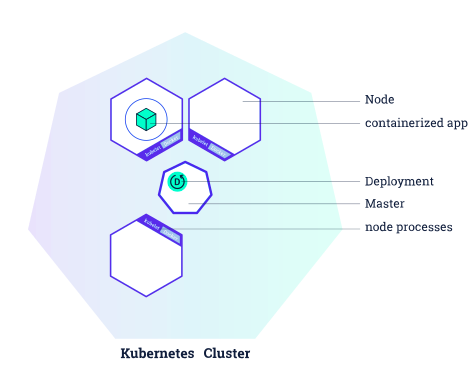
\includegraphics[scale=0.6]{img/module_02_first_app.png}
	\label{fig:controller}
	\caption{Controladores y servicios}
\end{figure}


Kubernetes automatiza la distribución y planificación de las aplicaciones contenerizadas sobre los
diferentes nodos del cluster de la forma más eficiente, intentando equilibrar el uso de recursos en cada
nodo. Al definir una aplicación en un cluster, el Master es el que recibiría la información a través de la
API de Kubernetes y desplegaría la aplicación en el worker que crea conveniente.

\subsubsection{Pod - la unidad mínima desplegable}

Un Pod es una abstracción de Kubernetes que representa la unidad mínima desplegable sobre el cluster. Cada Pod es un conjunto de una o más aplicaciones contenerizadas y algunos recursos compartidos entre estos contenedores. Estos recursos incluyen:
\begin{itemize}
	\item Almacenamiento compartido o volúmenes.
	\item Una dirección IP del cluster asignada al Pod.
	\item Información sobre cómo ejecutar cada uno de los contenedores, la imagen del contenedor, puertos abiertos, etc.
\end{itemize}


\begin{figure}
    \centering
	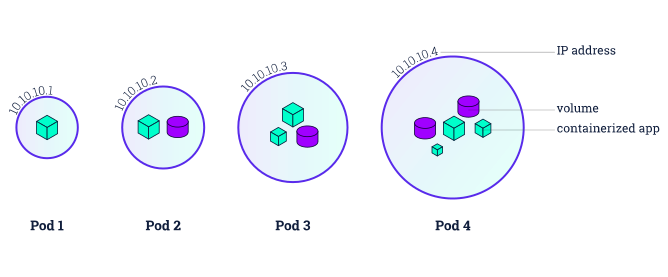
\includegraphics[scale=0.6]{img/module_03_pods.png}
	\label{fig:Pods}
	\caption{Pods}
\end{figure}

\subsubsection{Controladores}

Como hemos visto anteriormente, los Pods son la unidad mínima desplegable. A continuación se
explicará cómo estos recursos son generados y gestionados por diferentes tipos de controladores .
Un controlador, por tanto, es el encargado de generar estos Pods. Kubernetes proporciona diferentes
tipos para cubrir diferentes casos de uso. Los principales controladores que se utilizan son:

\begin{itemize}
	\item \textbf{ReplicaSet}: la función de este tipo de controlador es garantizar la disponibilidad de un determinado número específico de pods identicos (replicas). Este controlador no suele ser utilizado directamente.
	\item \textbf{Deployment}: representa el controlador más indicado para ejecutar aplicaciones stateless, es decir, aplicaciones que no guardan estado, por ejemplo: un proxy, un microservicio, etc. Es el controlador más común y uno de los más fáciles de utilizar. Su función es generar y gestionar diferentes ReplicaSet, estos ya serán los encargados de controlar los Pods generados.
	\item \textbf{StatefulSet}: al contrario que el deployment, este tipo de controlador es ideal para ejecutar aplicaciones stateful, o aplicaciones que guardan estado. Normalmente requieren identificación única a nivel de red por réplica y/o almacenamiento persistente. Algunos ejemplos son:
	\begin{itemize}
	    \item Bases de datos: MongoDB, Redis, PostgreSQL, MySQL, etc. 
	    \item Gestores de colas: Kafka, RabbitMQ, etc.
	    \item Gestores de configuración: Zookeeper, Consul, etc.
	\end{itemize}
	\item \textbf{DaemonSet}: la finalidad de este tipo de controlador es asegurar que un pod se ejecuta en cada nodo del cluster o en un conjunto específico de estos nodos. Algunos ejemplos son:
	\begin{itemize}
	    \item Demonios de Logging: Fluentd suele levantar un Pod en cada nodo con el fin de recopilar los logs de la salida estandard de los Pods que se ejecutan en ese nodo y mandarlos a una base de datos central de logs, normalmente a ElasticSearch.
	    \item Demonios de Monitoring: Prometheus Node Exporter suele ejecutar un pod en cada nodo con el find de facilitar la recogida de métricas a través de un servidor central de Prometheus.
	\end{itemize}
	\item \textbf{Jobs}: este tipo se utiliza para llevar a cabo una tarea específica utilizando un Pod y asegurarse que la tarea se completa satisfactoriamente. Cuando se lanza un job, se lanzan uno o varios pods   y si no se producen problemas durante su ejecución, se finalizará con éxito. Un ejemplo típico puede ser un backup de una base de datos en el que este pod se levantaría, haría un dump de la base de datos (en otro pod) y la guardaría en un volumen o en un Cloud Object Storage.
	\item \textbf{CronJobs}: adecuado para planificar y ejecutar tareas programadas. Este creará un Job que se ejecutará cada vez que llegue un momento específico definido en forma de crontab con el siguiente formato:
	\begin{itemize}
	    \item *(día 0-59) *(hora 0-23) *(día del mes 1-31) *(mes 1-12) *(día semana 0-6)
	    \item Un backup programado todos los días a las 4:30h sería:  [30 04 * * *] 
	\end{itemize}
\end{itemize}

\begin{figure}
    \centering
	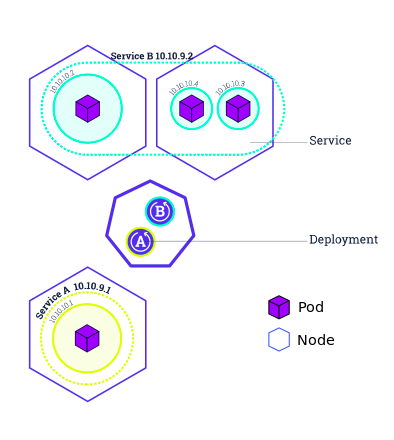
\includegraphics[scale=0.6]{img/module_04_services.png}
	\label{fig:controllers}
	\caption{Controladores y servicios}
\end{figure}

\subsubsection{Servicios}

Los Pods son entes lógicos que pueden morir en cualquier momento, de hecho, tienen su propio ciclo de vida. Cuando un nodo worker se pierde, se reinicia o se apaga, los Pods que se ejecutaban sobre este nodo son eliminados y posteriornente regenerados en otro nodo. Estos se pueden eliminar también manualmente mediante la línea de comandos, o en algunos casos son eliminados por el controlador que los genera, por ejemplo, cuando se reduce el número de réplicas de un Deployment.

Cada Pod tiene su propia dirección IP única y, cuando un pod muere, si se genera otra réplica similar  se le asignará otra IP diferente. También podríamos encontrar un controlador que crea varias réplicas de un mismo tipo de aplicación. Por tanto, existe una necesidad de disponer de una dirección que nos garantice el acceso a la aplicación con indiferencia del pod que atienda esta petición. Esta necesidad es cubierta por los servicios de Kubernetes. 

Un servicio es una abstracción que agrupa un conjunto de Pods y políticas relacionadas con el acceso a los mismos. Esta agrupación se realiza a través de Labels o etiquetas que se definen tanto en el controlador como en el servicio. Básicamente, el servicio expone los pods que tengan unas determinadas etiquetas.

Estos servicios facilitan un bajo nivel de acoplamiento (loose coupling) entre aplicaciones, como consecuencia de que la comunicación entre estas se realice a través de una IP asignada al servicio, independiente a la de los pods desplegados. Por ejemplo, una aplicación A que accede a una aplicación B podrá acceder a la IP del servicio B y finalmente se balanceará el tráfico sobre una de las diferentes réplicas de B.

También se ofrece descubrimiento de servicios o  service discovery a través de DNS. Básicamente se genera una entrada DNS por cada servicio siguiendo la siguiente estructura fully qualified domain (FQDN): svcName.namespace.svc.cluster.local. Por tanto, en el ejemplo anterior, la aplicación A podría llamar a ”B.default.svc.cluster.local” y se e resolvería como la IP del servicio B.

Los servicios también son muy importantes de cara a exponer las aplicaciónes fuera del cluster. A continuación se van a presentar los principales tipos que encontramos:

\begin{itemize}
	\item \textbf{ClusterIP}: este es el tipo por defecto. Expone la IP del servicio internamente en el cluster.
	
    \item \textbf{NodePort}: se forma sobre la clase ClusterIP, además de exponerse internamente, se realiza un NAT entre el puerto real del servicio y un puerto de los Nodos. Para acceder a una aplicación expuesta de esta forma se debería acceder a: IPNodo:NodePort.
    
    \item \textbf{LoadBalancer (LB)}: este tipo se construye sobre la clase NodePort. Solicita un balanceador de carga L4 a tu proveedor Cloud, cuando está disponible se asigna una IP externa al servicio y se abren los puertos declarados. Cuando una petición llega a esa IP y puerto del LB, este la traduce a un IPNodo:NodePort. Este LB balancea sobe los diferentes nodos del cluster.
\end{itemize}



\section{Helm - Package Manager}


\section{Istio - Service Mesh}

\section{Elastic Stack - Logging}

\section{PrometheusGrafana - Monitoring}

\section{Velero - Backup}

%%%%%%%%%%%%%%%%%%%%%%%%%%%%%%%%%%%%%%%%%%%%%%%%%%%%%%%%%%%%%%%%%%%%%%%%%%%%%%%%%
\chapter{PREPARACIÓN DEL ENTORNO}

\section{Entornos de prueba}

\subsection{Local - Minikube}

\subsection{IBM Cloud - IKS Lite}

\section{Diseño}

\subsection{Google Cloud - GKE}

\subsection{Componentes}

\section{Despliegue}

\section{Puesta en marcha}

%%%%%%%%%%%%%%%%%%%%%%%%%%%%%%%%%%%%%%%%%%%%%%%%%%%%%%%%%%%%%%%%%%%%%%%%%%%%%%%%%
\chapter{PRUEBAS DE CONCEPTO}

%%%%%%%%%%%%%%%%%%%%%%%%%%%%%%%%%%%%%%%%%%%%%%%%%%%%%%%%%%%%%%%%%%%%%%%%%%%%%%%%%
\chapter{CONCLUSIONES Y PROPUESTAS}


\section{Conclusiones}



\section{Trabajo futuro}

\nocite{*}
\bibliographystyle{TFMbibstyle}
\bibliography{TFMbibliografia}


%\renewcommand{\refname}{BIBLIOGRAFÍA}
%\bibliographystyle{jmb}
%\bibliography{mibibliografia}

\addcontentsline{toc}{chapter}{BIBLIOGRAFIA}

\chapter*{CONTENIDO DEL CD}
En el contenido del CD que acompaña a la memoria podemos encontrar los
siguientes recursos:
\begin{itemize}
 \item Memoria del trabajo en los formatos PDF, DOCX y DOC dentro del directorio
Memoria.
 \item Código fuente del trabajo dentro del directorio Código fuente.
 \item Libros y artículos a los que se ha hecho referencia durante la memoria y que se han
utilizado como bibliografía. Los cuales podemos encontrar en el directorio
Bibliografía.
 \item Páginas Web que han servido de bibliografía. Las podemos encontrar dentro del
directorio Bibliografia/Enlaces Web.
 \item Manual de usuario de la aplicación junto con ejemplos, que podemos encontrar en
el directorio Manual y ejemplos.
\end{itemize}

\addcontentsline{toc}{chapter}{CONTENIDO DEL CD}

\appendix

\chapter{CLUSTER LOCAL EN MINIKUBE}

\chapter{CLUSTER IKS LITE EN IBM CLOUD}

\chapter{CLUSTER GKE EN GOOGLE CLOUD}

\chapter{CLUSTER IKS EN IBM CLOUD}


\end{document}
